\subsection{Versuchsaufbau}
\label{sec:Versuchsaufbau}
\begin{figure}
  \centering
  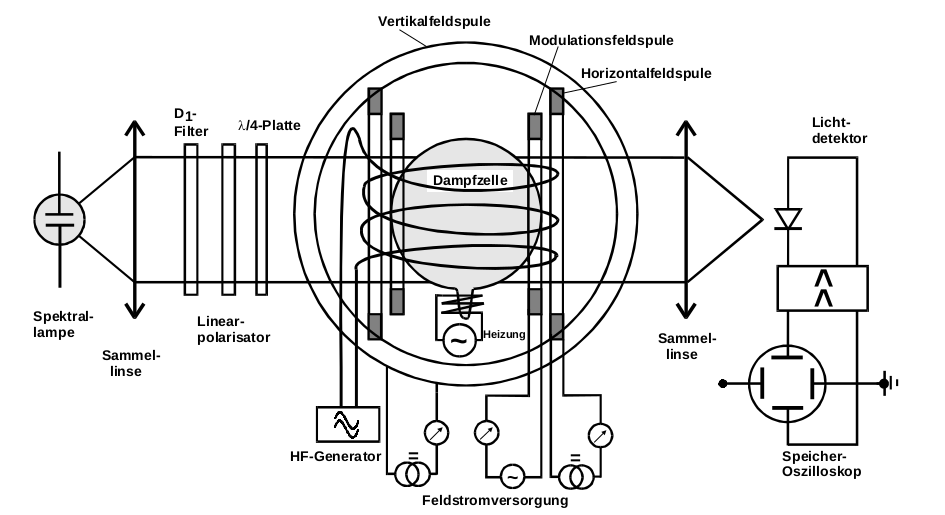
\includegraphics[width=0.9\columnwidth]{pictures/aufbau.png}
  \caption{Prinzipieller Aufbau des Versuchs.\cite{Anleitung}}
  \label{fig:aufbau}
\end{figure}

Der prinzipielle Aufbau des Versuches ist in Abbildung \ref{fig:aufbau}
zu sehen.
Als Lichtquelle wird eine Rb-Spektrallampe verwendet.
Das Licht aus der Spektrallampe trifft zuerst auf eine Sammellinse
zur Fokussierung und dann auf einen
D$_1$-Filter, der die D$_1$-Linie aus dem Rubidium-Spektrum
($\lambda = \SI{794,8}{\nano\meter}$) passieren lässt und so das
notwendige D$_1$-Licht erzeugt. Die rechtszirkulare Polarisation
wird durch den darauffolgenden Polarisationsfilter und eine $\frac{\lambda}{4}$-Platte ermöglicht.
In der Dampfzelle befindet sich der Rb-Dampf, der mit einem Ofen geheizt
wird. An der Dampfzelle sind drei Helmholtz-Spulenpaare zur Erzeugung von
Magnetfeldern angebracht. Eins ist vertikal ausgerichtet
($R=\SI{11,735}{\centi\meter}, N=20$) und dient
zum Ausgleich der Vertikalkomponente des Erdmagnetfeldes.
Die anderen beiden Spulenpaare erzeugen horizontale Magnetfelder und sind
aufeinander aufgewickelt. Es handelt sich um die Sweep-Spule ($R=\SI{16,39}{\centi\meter}, N=11$) mit variierbarem Spulenstrom und die
Horizontalfeld-Spule ($R=\SI{15,79}{\centi\meter}, N=154$).
Außerdem ist durch die RF-Spule noch ein Helmholtz-Spulenpaar gegeben, welches das
Wechselfeld zur Anregung der induzierten Emission erzeugt.

Für die Transparenzmessung ist hinter der Dampfzelle wieder eine Sammellinse zur Fokussierung
des D$_1$-Lichtes auf einen Lichtdetektor angebracht. Der Lichtdetektor ist an einen Eingang
eines Oszilloskopes angeschlossen.
An einer Kontrollvorrichtung können alle Spulenströme, sowie der Startwert des horizontalen
Magnetfeldes und die Dauer eines Durchlaufes eingestellt werden.
